\begin{figure}[!ht] 
\label{fig:solutions/1/8/triangle_abc}
\centering
\resizebox{\columnwidth}{!}{%\documentclass{standalone}
%
%\usepackage{tikz,pgf} %and any other packages or tikzlibraries your picture needs
%
%\begin{document}
%\resizebox{\columnwidth}{!}{
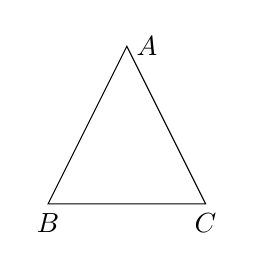
\begin{tikzpicture}
\draw (0,0) node[anchor=north]{$B$}
  -- (1,2) node[anchor=west]{$A$}
  -- (2,0) node[anchor=north]{$C$}
  -- cycle;
\end{tikzpicture}
%}
%\end{document}}
\caption{$\triangle ABC$}
\end{figure}
Given that two angles of traingle are equal,
\begin{align}
    \label{eq:solutions/1/8/1}\angle{ABC}&=\angle{ACB}\\[5pt]
\cos\angle{ABC} &= \cos\angle{ACB}\\[5pt]
    \label{eq:solutions/1/8/2}\frac{(\vec{B}-\vec{A})^T(\vec{B}-\vec{C})}{\norm{\vec{B}-\vec{A}}\norm{\vec{B}-\vec{C}}} &= \frac{(\vec{C}-\vec{A})^T(\vec{C}-\vec{B})}{\norm{\vec{C}-\vec{A}}\norm{\vec{C}-\vec{B}}}\\[7pt]
    \label{eq:solutions/1/8/3}\frac{(\vec{B}-\vec{A})^T(\vec{B}-\vec{C})}{\norm{\vec{B}-\vec{A}}} &= \frac{(\vec{C}-\vec{A})^T(\vec{C}-\vec{B})}{\norm{\vec{C}-\vec{A}}}
\end{align}
It can be showed that,
% \norm{\vec{B}}^2 - \vec{B}^T\vec{C} - \vec{A}^T\vec{B} + \vec{A}^T\vec{C}
% $\norm{\vec{B}}^2 = \norm{\vec{A}-\vec{B}}^2 - \norm{\vec{A}}^2 + 2\vec{A}^T\vec{B}$
\begin{multline}
    \label{eq:solutions/1/8/4}
(\vec{B}-\vec{A})^T(\vec{B}-\vec{C}) = \norm{\vec{A}-\vec{B}}^2 - (\vec{A}-\vec{C})^T(\vec{A}-\vec{B})
\end{multline}
\begin{multline}
    \label{eq:solutions/1/8/5}(\vec{C}-\vec{A})^T(\vec{C}-\vec{B}) = \norm{\vec{A}-\vec{C}}^2 - (\vec{A}-\vec{C})^T(\vec{A}-\vec{B})
\end{multline}
Substituting \eqref{eq:solutions/1/8/4} and \eqref{eq:solutions/1/8/5} in \eqref{eq:solutions/1/8/3},
{\footnotesize
\begin{align}
\label{eq:solutions/1/8/6}\frac{\norm{\vec{A}-\vec{B}}^2 - (\vec{A}-\vec{C})^T(\vec{A}-\vec{B})}{\norm{\vec{B}-\vec{A}}}&=\frac{\norm{\vec{A}-\vec{C}}^2 - (\vec{A}-\vec{C})^T(\vec{A}-\vec{B})}{\norm{\vec{C}-\vec{A}}}\\
\label{eq:solutions/1/8/7}\norm{\vec{A}-\vec{B}} - \frac{(\vec{A}-\vec{C})^T(\vec{A}-\vec{B})}{\norm{\vec{B}-\vec{A}}}&=\norm{\vec{A}-\vec{C}} - \frac{(\vec{A}-\vec{C})^T(\vec{A}-\vec{B})}{\norm{\vec{C}-\vec{A}}}\\
\label{eq:solutions/1/8/8}\norm{\vec{A}-\vec{B}} - \norm{\vec{A}-\vec{C}} \cos{\angle{BAC}}&=\norm{\vec{A}-\vec{C}} - \norm{\vec{A}-\vec{B}} \cos{\angle{CAB}}\\
\label{eq:solutions/1/8/9}\norm{\vec{A}-\vec{B}} +  \norm{\vec{A}-\vec{B}} \cos{\angle{CAB}}&=\norm{\vec{A}-\vec{C}} + \norm{\vec{A}-\vec{C}} \cos{\angle{BAC}}\\
\label{eq:solutions/1/8/10}\norm{\vec{A}-\vec{B}}(1 + \cos{\angle{CAB}})&=\norm{\vec{A}-\vec{C}}(1 + \cos{\angle{BAC}})\\
\implies\norm{\vec{A}-\vec{B}} &= \norm{\vec{A}-\vec{C}}
\end{align}
}
